\documentclass[9pt]{beamer}
\usepackage{beamerthemeFrankfurt}
\usepackage{amsmath}
\usepackage{graphicx}
\usepackage[T1]{fontenc}
\usepackage{xcolor}
\usepackage[frenchb]{babel}
\usepackage[utf8]{inputenc}
\usecolortheme{seagull}
\usefonttheme{serif}
\useoutertheme{shadow}

\title{Messages}
\institute{University of Orléans}
\date{\today}

\setbeamertemplate{blocks}[rounded][shadow=false]
\setbeamercolor{background canvas}{bg=blue!20}

\begin{document}

\begin{frame}
	\titlepage
\end{frame}

\begin{frame}
	\frametitle{Presentation}
	\begin{center} 
		\begin{itemize}
			\item Class of messages
			\item Format of messages
			\item Message class
			\item Messages track
		 \end{itemize}
	 \end{center}
\end{frame}

\begin{frame}
	\frametitle{Class of messages}
	\setbeamercolor{block title}{fg=black, bg=blue!50}
	\setbeamercolor{block body}{fg=black, bg=red!10}
	\begin{block}{Six class}
		There is six different class of messages that may be throw:
		\begin{itemize}
			\item<2-> CS : client service message.
			\item<3-> CG : client game message.
			\item<4-> SS : server service message.
			\item<5-> SG : server game message.
			\item<6-> SP : server problem message.
			\item<7-> SR : server recall message.
		\end{itemize}
	\end{block}
	\begin{block}{Example of utilisation}
		\begin{itemize}
			\item<7-> MessageCS.connect() : message to request a connection.
			\item<8-> MessageSR.types : messages with all the types of the player.
		\end{itemize}
	\end{block}
	\transdissolve
\end{frame}

\begin{frame}
	\frametitle{Format of messages}
	\setbeamercolor{block title}{fg=black, bg=blue!50}
	\setbeamercolor{block body}{fg=black, bg=red!10}
	\begin{block}{Same for all}
		A message is represented by a string.
		All messages can be represented by four properties.
		\begin{itemize}
			\item ip : the ip of the client or server
			\item port : the port of the client or server
			\item type : the type of message
			\item parameters : the message datas.
		\end{itemize}
	\end{block}
	\begin{block}{A separator in top}
		To represent a message we use an auto generated separator.
		The final format is as follow:
		SEPA+Ip+SEPA+port+SEPA+type+SEPA+Parameters+SEPA.
	\end{block}
	\transdissolve
\end{frame}

\begin{frame}
	\frametitle{Format of messages}
	\setbeamercolor{block title}{fg=black, bg=blue!50}
	\setbeamercolor{block body}{fg=black, bg=red!10}

	\begin{block}{Parameters : different for all}
		The parameter format must be generic because there is message with no limit of parameters or even no parameters.
	\end{block}

	\begin{block}{A separator inside another}
		To represent the parameters we will then uses another auto-generate and different separator.
		The final format is as follow:
		SEPA+Param1+SEPA+Param2+SEPA+...+ParamN+SEPA.
	\end{block}

	\begin{block}{Example of message}
		Main: SEP\color{red}165.165.165.165\color{black}SEP\color{red}4444\color{black}SEP\color{red}sg\_chat\color{black}SEP\color{red}Parameters\color{black}SEP
		Parameters: SEP2\color{red}playername\color{black}SEP2\color{red}message\color{black}SEP2
	\end{block}
	\transdissolve
\end{frame}

\begin{frame}
	\frametitle{ Message class }
	\setbeamercolor{block title}{fg=black, bg=blue!50}
	\setbeamercolor{block body}{fg=black, bg=red!10}

	\begin{block}{The main : Message}
		This class contains the methods to build message. The important one are :
		\begin{itemize}
			\item<2->  new\_separator : generate a new separator
			\item<3-> getParam : return a parameter in a type with a limit of parameters.
			\item<4-> getListeParam : return a list in a type with no limit of parameters.
			\item<5->  isMessage : return true if a message respect the format.
		\end{itemize}
		And the one that will be modified when a new message is created:
		\begin{itemize}
			\item<6-> isTypeListParam : return true for no limit params message.
			\item<7-> isNotTypeListParam : the opposite.
			\item<8-> getTailleTypeMessage : return the number of params.
		\end{itemize}
	\end{block}
	\begin{block}{Note}
		\begin{itemize}
			\item<9-> \color{red} We use static method and not object because we manage string for the messages.
		\end{itemize}
	\end{block}
	\transdissolve
\end{frame}

\begin{frame}
	\frametitle{ Message class }
	\setbeamercolor{block title}{fg=black, bg=blue!50}
	\setbeamercolor{block body}{fg=black, bg=red!10}

	\begin{block}{MessageType for each type}
		For each of the six types(SG...etc) there is a class.
		Each type of message will be represent by :
		\begin{itemize}
			\item<2->  A static and public name starting by SG, SS...etc
			\item<3-> Example: \color{red} SG\_CHAT\_NAME="sg\_chat"
			\item<2->  A static and public integer which specifies the number of parameters.
			\item<4-> Example: \color{red} SG\_CHAT\_NUM\_PARAMS=4;
			\item<2->  A static and public integer for each parameter
			\item<5-> Example: \color{red} SG\_CHAT\_MESSAGE = 4;
			\item<2->  A static and public method 
			\item<6-> Example: When call :\color{red} MessageSG.chat(...)
		\end{itemize}
	\end{block}
	\transdissolve
\end{frame}

\begin{frame}
	\frametitle{ Message class }
	\setbeamercolor{block title}{fg=black, bg=blue!50}
	\setbeamercolor{block body}{fg=black, bg=red!10}

	\begin{block}{Two interfaces}
		The problem with this generic messages is that they will be many messages
		to handle.
		So to simplify and not forget the method two interface exists:
		\begin{itemize}
			\item onMessageReceived: contains one method for each message type with no parameter.
			\item setMessageSend: contains one method for each message with the parameters of the type of message.
		\end{itemize}
	\end{block}
	\begin{block}{MessageManager : A usefull class}
		A MessageManager will implements the two interface. \\
		To manage messages we build a class wich extends it and will :
		\begin{itemize}	
			\item implement a setMethod to send message.
			\item implement a onMethod to manage the receive messages.
		\end{itemize}
	\end{block}
	\transdissolve
\end{frame}

\begin{frame}
	\begin{Huge}
		Messages Track !
	\end{Huge}
\end{frame}


\begin{frame}
	\frametitle{CS and SSNewGame Message}
 	\centerline{ 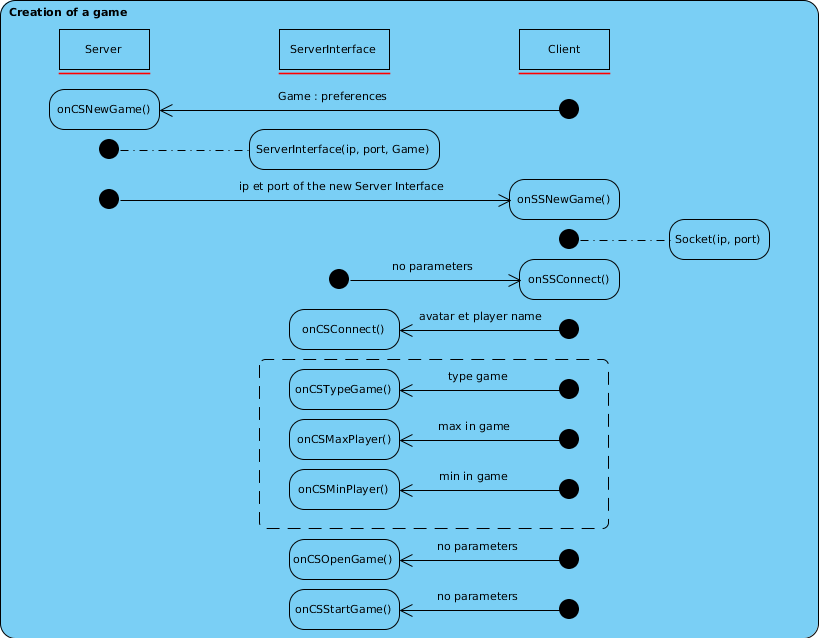
\includegraphics[width=11cm, height=7.5cm]{gamecreation.png}}
	%\includegraphics[width= 0.7\linewidth]{game_creation_mini.png}
	\transdissolve
\end{frame}

\begin{frame}
	\frametitle{Reconnection first part}
 	\centerline{ 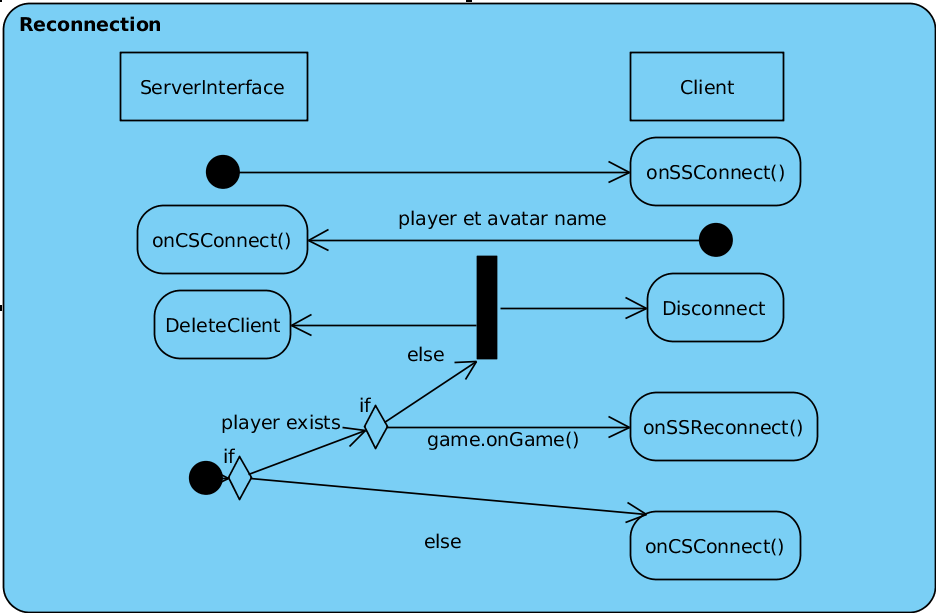
\includegraphics[width=11cm, height=7.5cm]{reconnection.png}}
	%\includegraphics[width= 0.7\linewidth]{game_creation_mini.png}
	\transdissolve
\end{frame}

\begin{frame}
	\frametitle{Reconnection second part}
 	\centerline{ 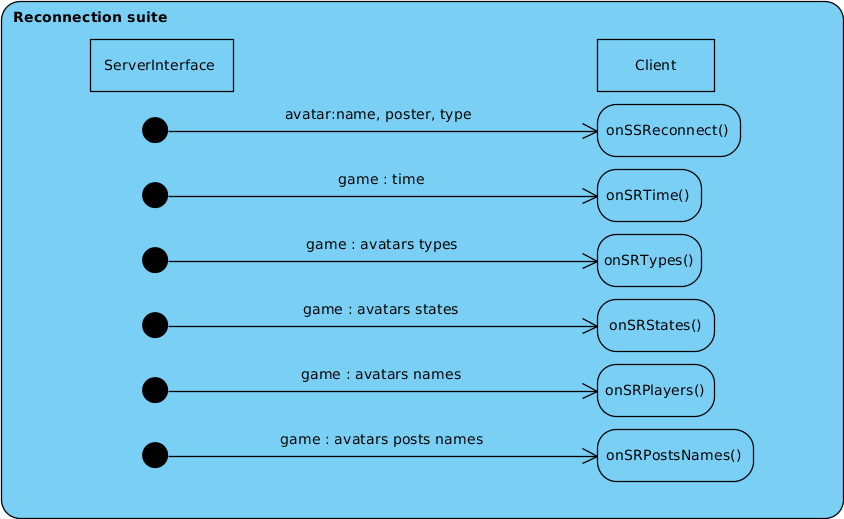
\includegraphics[width=11cm, height=7.5cm]{reconnectionsuite.png}}
	%\includegraphics[width= 0.7\linewidth]{game_creation_mini.png}
	\transdissolve
\end{frame}

\end{document}
